\documentclass[11pt]{article}
\usepackage[margin=1in]{geometry}
\usepackage{amsmath, amssymb, amsfonts}
\usepackage{booktabs}
\usepackage{enumitem}
\usepackage{microtype}
\usepackage{hyperref}
\usepackage{pgfplots}
\pgfplotsset{compat=1.16}
\setlist[enumerate]{leftmargin=*}

\newcommand{\dd}{\,\mathrm{d}}

\title{Tutorial 1}
\author{ECON 101 -- Macroeconomics}
\date{Fall 2025}


\begin{document}
\maketitle



\section*{Part A. Numerical Problems}

\textbf{Q1. Market Equilibrium and Price Controls}\\
The market for coffee is:
\[
Q_d = 100 - 2P, \qquad Q_s = 20 + 3P.
\]
\begin{enumerate}[label=(\alph*)]
\item Find the equilibrium price and quantity.
\item With a price floor of $P=20$, compute the surplus (if any).
\item With a price ceiling of $P=10$, compute the shortage (if any).
\end{enumerate}

\bigskip

\noindent \textbf{Q2. Demand Shift from Income}\\
Demand for laptops is
\[
Q_d = 500 - 5P + 0.5Y
\]
and supply is
\[
Q_s = 100 + 3P.
\]
\begin{enumerate}[label=(\alph*)]
\item If $Y=200$, find the equilibrium $P$ and $Q$.
\item If $Y=300$, find the new equilibrium $P$ and $Q$.
\item Briefly interpret how the income change affects equilibrium.
\end{enumerate}

\bigskip

\noindent \textbf{Q3. Point Elasticity and Revenue}\\
Demand is
\[
Q_d = 200 - 4P.
\]
\begin{enumerate}[label=(\alph*)]
\item Compute the price elasticity of demand at $P=30$.
\item Classify demand at that price (elastic, inelastic, unit elastic).
\item What happens to total revenue if price increases slightly from $P=30$?
\end{enumerate}

\section*{Part B. Graphical Problems}

\textbf{Q4. Supply Shock (Graphical and Numerical)}\\
Initial demand and supply:
\[
Q_d = 80 - 2P, \qquad Q_s = 10 + 2P.
\]
\begin{enumerate}[label=(\alph*)]
\item Graph $Q_d$ and $Q_s$; mark the initial equilibrium.
\item An input cost increase shifts supply to $Q_s' = -10 + 2P$. Graph $Q_s'$ on the same axes and identify the new equilibrium.
\item State the direction of the changes in equilibrium $P$ and $Q$ and why.
\end{enumerate}

\begin{center}
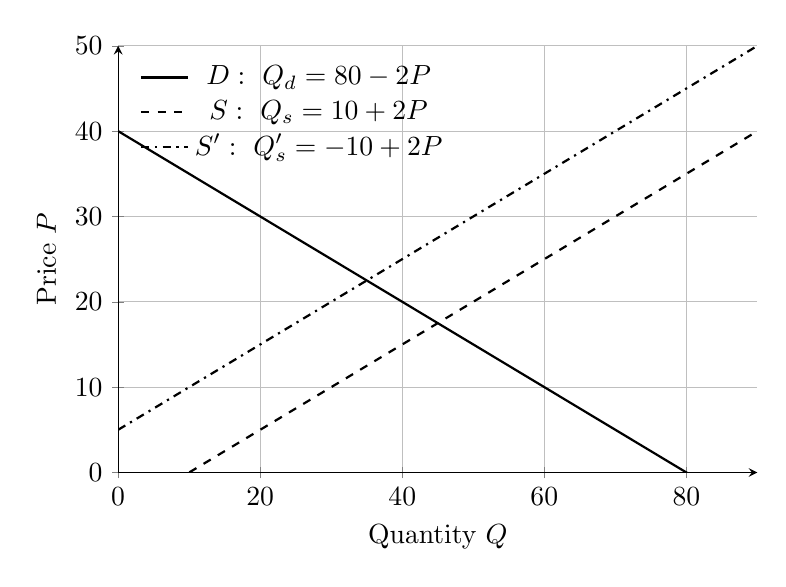
\begin{tikzpicture}
\begin{axis}[
  width=0.8\textwidth, height=7cm,
  axis lines=left, xlabel={Quantity $Q$}, ylabel={Price $P$},
  xmin=0, xmax=90, ymin=0, ymax=50, samples=2, domain=0:90,
  legend style={at={(0.02,0.98)},anchor=north west, draw=none, fill=none},
  grid=both
]
% Invert functions to P(Q) for plotting: Q_d = 80 - 2P -> P = (80 - Q)/2
\addplot[thick] {(80 - x)/2};
\addlegendentry{$D:~Q_d=80-2P$}
% Q_s = 10 + 2P -> P = (Q - 10)/2
\addplot[thick, dashed] {(x - 10)/2};
\addlegendentry{$S:~Q_s=10+2P$}
% shifted supply: Q_s' = -10 + 2P -> P = (Q + 10)/2
\addplot[thick, dashdotted] {(x + 10)/2};
\addlegendentry{$S':~Q_s'=-10+2P$}
\end{axis}
\end{tikzpicture}
\end{center}

\bigskip

\noindent \textbf{Q5. Rent Ceiling (Graphical and Numerical)}\\
Rental housing market:
\[
Q_d = 120 - 2P, \qquad Q_s = 20 + 2P.
\]
\begin{enumerate}[label=(\alph*)]
\item Graph $D$ and $S$ and mark the competitive equilibrium.
\item Impose a rent ceiling at $P=20$. On the graph, show the shortage.
\item Compute the numerical size of the shortage.
\end{enumerate}

\begin{center}
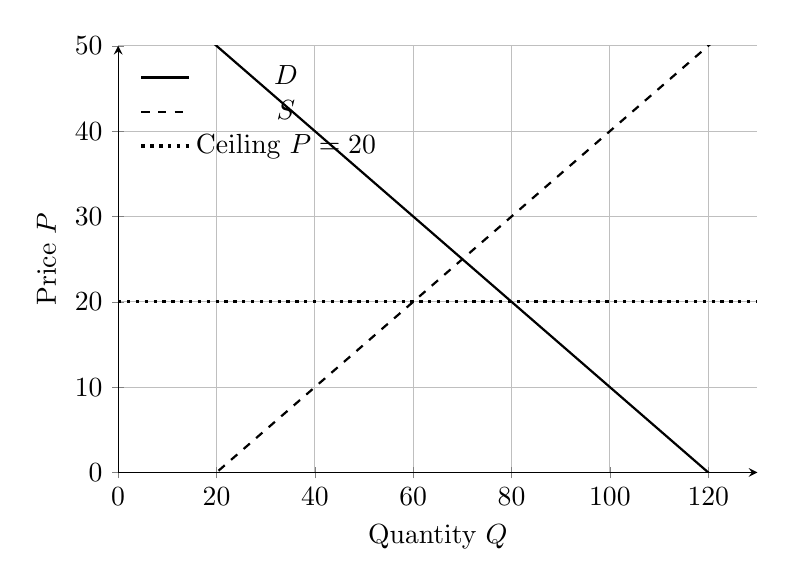
\begin{tikzpicture}
\begin{axis}[
  width=0.8\textwidth, height=7cm,
  axis lines=left, xlabel={Quantity $Q$}, ylabel={Price $P$},
  xmin=0, xmax=130, ymin=0, ymax=50, samples=2, domain=0:130,
  legend style={at={(0.02,0.98)},anchor=north west, draw=none, fill=none},
  grid=both
]
% P(Q) forms:
% Q_d=120-2P -> P=(120-Q)/2
\addplot[thick] {(120 - x)/2};
\addlegendentry{$D$}
% Q_s=20+2P -> P=(Q-20)/2
\addplot[thick, dashed] {(x - 20)/2};
\addlegendentry{$S$}
% Price ceiling line at P=20
\addplot[very thick, dotted, domain=0:130] {20};
\addlegendentry{Ceiling $P=20$}
\end{axis}
\end{tikzpicture}
\end{center}

\bigskip

\noindent  \textbf{Q6. Comparative Statics: Demand Increase}\\
Wheat market:
\[
Q_d = 600 - 10P, \qquad Q_s = 100 + 5P.
\]
\begin{enumerate}[label=(\alph*)]
\item Solve for the initial equilibrium.
\item Demand increases to $Q_d' = 700 - 10P$. Find the new equilibrium.
\item On a diagram, show the shift and both equilibria. Briefly explain the changes.
\end{enumerate}

\begin{center}
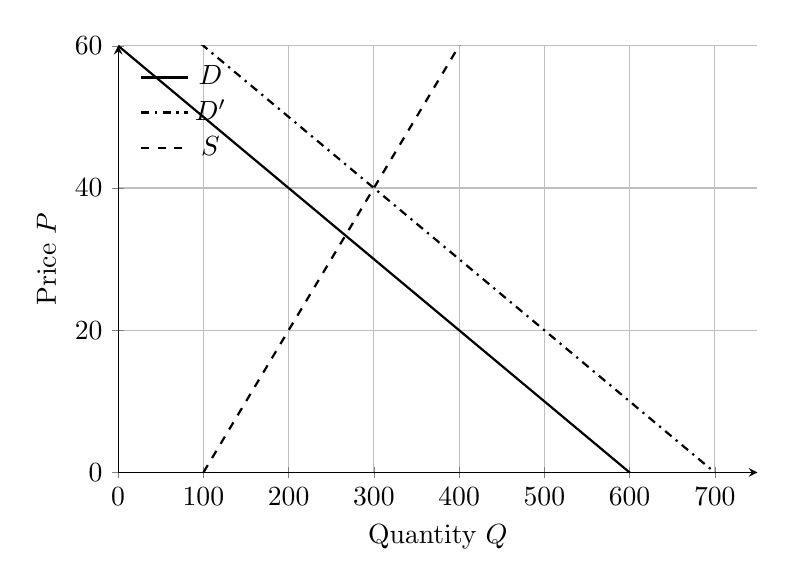
\begin{tikzpicture}
\begin{axis}[
  width=0.8\textwidth, height=7cm,
  axis lines=left, xlabel={Quantity $Q$}, ylabel={Price $P$},
  xmin=0, xmax=750, ymin=0, ymax=60, samples=2, domain=0:750,
  legend style={at={(0.02,0.98)},anchor=north west, draw=none, fill=none},
  grid=both
]
% P(Q) forms:
% D: Q=600-10P -> P=(600-Q)/10
\addplot[thick] {(600 - x)/10};
\addlegendentry{$D$}
% D': Q=700-10P -> P=(700-Q)/10
\addplot[thick, dashdotted] {(700 - x)/10};
\addlegendentry{$D'$}
% S: Q=100+5P -> P=(Q-100)/5
\addplot[thick, dashed] {(x - 100)/5};
\addlegendentry{$S$}
\end{axis}
\end{tikzpicture}
\end{center}

\newpage
\section*{Solutions}

\textbf{Q1.}
\begin{enumerate}[label=(\alph*)]
\item $100-2P=20+3P \Rightarrow 80=5P \Rightarrow P^\ast=16,\; Q^\ast=68.$
\item At $P=20$: $Q_d=100-40=60,\; Q_s=20+60=80 \Rightarrow \text{surplus}=20.$
\item At $P=10$: $Q_d=100-20=80,\; Q_s=20+30=50 \Rightarrow \text{shortage}=30.$
\end{enumerate}

\bigskip

\textbf{Q2.}
\begin{enumerate}[label=(\alph*)]
\item $Y=200 \Rightarrow Q_d=500-5P+100=600-5P.$\\
$600-5P=100+3P \Rightarrow 500=8P \Rightarrow P^\ast=62.5.$\\
$Q^\ast=100+3(62.5)=287.5.$
\item $Y=300 \Rightarrow Q_d=500-5P+150=650-5P.$\\
$650-5P=100+3P \Rightarrow 550=8P \Rightarrow P^{\ast\prime}=68.75.$\\
$Q^{\ast\prime}=100+3(68.75)=306.25.$
\item Income rises, demand shifts right. For a normal good, both $P$ and $Q$ increase.
\end{enumerate}

\bigskip

\textbf{Q3.}
\begin{enumerate}[label=(\alph*)]
\item $Q=200-4P.$ At $P=30$, $Q=80.$\\
$\dfrac{\dd Q}{\dd P}=-4.$ Elasticity $\varepsilon = \left(\dfrac{\dd Q}{\dd P}\right)\left(\dfrac{P}{Q}\right)=(-4)\left(\dfrac{30}{80}\right)=-1.5.$
\item $|\varepsilon|=1.5>1 \Rightarrow$ demand is elastic at $P=30.$
\item When demand is elastic, a price increase reduces total revenue; TR falls from a marginal increase in $P$ at $P=30.$
\end{enumerate}

\bigskip

\textbf{Q4.}
\begin{enumerate}[label=(\alph*)]
\item $80-2P=10+2P \Rightarrow 70=4P \Rightarrow P^\ast=17.5,\; Q^\ast=80-2(17.5)=45.$
\item With $Q_s'=-10+2P$: $80-2P=-10+2P \Rightarrow 90=4P \Rightarrow P^{\ast\prime}=22.5,\; Q^{\ast\prime}=80-2(22.5)=35.$
\item Higher input costs shift supply left, raising $P$ and reducing $Q.$
\end{enumerate}

\bigskip

\textbf{Q5.}
\begin{enumerate}[label=(\alph*)]
\item $120-2P=20+2P \Rightarrow 100=4P \Rightarrow P^\ast=25,\; Q^\ast=70.$
\item With a ceiling at $P=20$: $Q_d=120-40=80,\; Q_s=20+40=60.$
\item Shortage $=Q_d-Q_s=20.$
\end{enumerate}

\bigskip

\textbf{Q6.}
\begin{enumerate}[label=(\alph*)]
\item $600-10P=100+5P \Rightarrow 500=15P \Rightarrow P^\ast=\frac{500}{15}\approx 33.33,\; Q^\ast=600-10(33.33)\approx 266.67.$
\item With $Q_d'=700-10P$: $700-10P=100+5P \Rightarrow 600=15P \Rightarrow P^{\ast\prime}=40,\; Q^{\ast\prime}=700-10(40)=300.$
\item Rightward demand shift raises both equilibrium price and quantity as buyers are willing to purchase more at each price.
\end{enumerate}

\end{document}
